\documentclass[border=3pt,tikz]{standalone}
% Shared look for every TikZ figure in these notes.
% Included by each standalone figure file; also keeps the figures consistent
% with the colours used in the PDF and on the website.

\usepackage{tikz}
\usepackage{pgfplots}
\pgfplotsset{compat=1.18}
\usetikzlibrary{arrows.meta, decorations.markings, decorations.pathmorphing,
                patterns, calc, positioning}
\usepackage{amsmath}

% Series colours are the three validated categorical slots also used by the
% interactive widgets, so a path drawn in the printed notes and the same path on
% the website are the same colour. They clear the colour-vision-deficiency and
% contrast checks as a set; every path is direct-labelled as well, so colour is
% never the only thing carrying identity.
\definecolor{duPurple}{HTML}{68246D}
\definecolor{duBlue}{HTML}{2A78D6}
\definecolor{duRed}{HTML}{EB6834}
\definecolor{duGreen}{HTML}{1BAF7A}
\definecolor{duGrey}{HTML}{6B6B6B}

\tikzset{
  axisline/.style   = {-{Stealth[length=3mm]}, line width=0.7pt, black},
  path1/.style      = {duBlue,   line width=1.1pt},
  path2/.style      = {duRed,    line width=1.1pt},
  path3/.style      = {duGreen,  line width=1.1pt},
  statedot/.style   = {circle, fill=black, inner sep=1.4pt},
  arrowhead/.style  = {decoration={markings,
                        mark=at position #1 with {\arrow{Stealth[length=2.6mm]}}},
                       postaction={decorate}},
  lbl/.style        = {font=\small},
  slbl/.style       = {font=\footnotesize, duGrey},
  workfill/.style   = {duPurple, opacity=0.16},
}

\usetikzlibrary{shapes.geometric, shapes.arrows}
\definecolor{heatc}{HTML}{D99694}
\definecolor{workc}{HTML}{00B050}
\definecolor{engine}{HTML}{BFBFBF}
\begin{document}
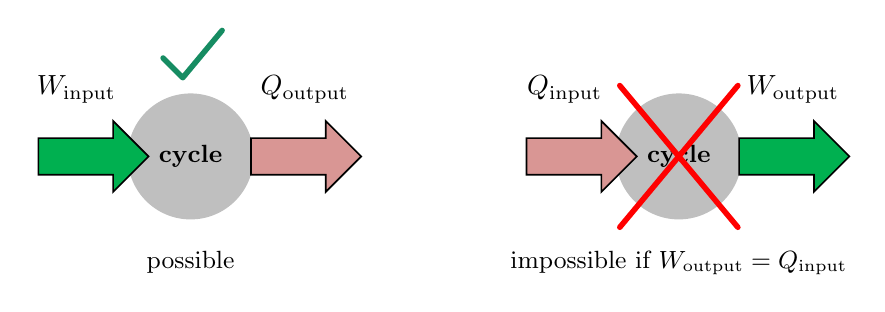
\begin{tikzpicture}[
  cyc/.style={circle, fill=engine, minimum size=1.6cm, font=\small\bfseries},
  blk/.style={single arrow, draw=black, line width=0.6pt, minimum height=1.4cm,
              minimum width=0.9cm, single arrow head extend=0.12cm}]
  % possible
  \node[cyc] (A) at (0,0) {cycle};
  \node[blk, fill=workc] at (-1.35,0) {};
  \node[blk, fill=heatc] at (1.35,0) {};
  \node[font=\normalsize] at (-1.45,0.85) {$W_\text{input}$};
  \node[font=\normalsize] at (1.45,0.85) {$Q_\text{output}$};
  \node[font=\small, align=center] at (0,-1.35) {possible};
  \draw[duGreen!80!black, line width=2pt, line cap=round, line join=round]
    (-0.35,1.25) -- (-0.1,1.0) -- (0.4,1.6);
  % impossible
  \begin{scope}[xshift=6.2cm]
    \node[cyc] (B) at (0,0) {cycle};
    \node[blk, fill=heatc] at (-1.35,0) {};
    \node[blk, fill=workc] at (1.35,0) {};
    \node[font=\normalsize] at (-1.45,0.85) {$Q_\text{input}$};
    \node[font=\normalsize] at (1.45,0.85) {$W_\text{output}$};
    \draw[red, line width=2pt, line cap=round] (-0.75,-0.9) -- (0.75,0.9);
    \draw[red, line width=2pt, line cap=round] (-0.75,0.9) -- (0.75,-0.9);
    \node[font=\small, align=center] at (0,-1.35)
      {impossible if $W_\text{output} = Q_\text{input}$};
  \end{scope}
\end{tikzpicture}
\end{document}
